\documentclass[11pt,a4paper]{article}
\usepackage[margin=1in]{geometry}
\usepackage{amsmath}
\usepackage{amssymb}
\usepackage{titlesec}
\usepackage{enumitem}
\usepackage{xcolor}
\usepackage[most]{tcolorbox}
\usepackage{fancyhdr}
\usepackage{listings}
\usepackage{hyperref}
\usepackage{graphicx}
\usepackage{tikz}
\usetikzlibrary{shapes.geometric, arrows, positioning, fit, backgrounds}
\usetikzlibrary{calc} 

\newcommand{\wrongmark}{\times}
\usepackage[utf8]{inputenc}
\usepackage{newunicodechar} 
\newunicodechar{✓}{\checkmark}
\newunicodechar{✗}{\wrongmark}
\DeclareUnicodeCharacter{2502}{|}
\DeclareUnicodeCharacter{251C}{+}
\DeclareUnicodeCharacter{2500}{-}
\DeclareUnicodeCharacter{2514}{+}

% Header and Footer
\pagestyle{fancy}
\fancyhf{}
\rhead{FastAPI Complete Guide}
\lhead{API Development for ML}
\cfoot{\thepage}

% Title formatting
\titleformat{\section}{\Large\bfseries\color{blue!70!black}}{\thesection}{1em}{}[\titlerule]
\titleformat{\subsection}{\large\bfseries\color{blue!50!black}}{\thesubsection}{1em}{}
\titleformat{\subsubsection}{\normalsize\bfseries\color{blue!40!black}}{\thesubsubsection}{1em}{}

% Code styling
\definecolor{codebg}{gray}{0.95}
\definecolor{codegreen}{rgb}{0,0.6,0}
\definecolor{codegray}{rgb}{0.5,0.5,0.5}
\definecolor{codepurple}{rgb}{0.58,0,0.82}

\lstdefinestyle{pythonstyle}{
    language=Python,
    backgroundcolor=\color{codebg},
    commentstyle=\color{codegreen},
    keywordstyle=\color{blue},
    numberstyle=\tiny\color{codegray},
    stringstyle=\color{codepurple},
    basicstyle=\ttfamily\small,
    breaklines=true,
    captionpos=b,
    keepspaces=true,
    numbers=left,
    numbersep=5pt,
    showspaces=false,
    showstringspaces=false,
    showtabs=false,
    tabsize=4,
    frame=single,
    xleftmargin=2em,
    framexleftmargin=1.5em
}

\lstdefinestyle{bashstyle}{
    language=bash,
    backgroundcolor=\color{codebg},
    basicstyle=\ttfamily\small,
    breaklines=true,
    frame=single,
    xleftmargin=2em,
    framexleftmargin=1.5em
}

\lstset{style=pythonstyle}

% Command box
\newtcolorbox{cmdbox}{
    colback=codebg,
    colframe=black!50,
    boxrule=0.5pt,
    left=2mm,
    right=2mm,
    top=1mm,
    bottom=1mm,
    breakable
}

% Example box
\newtcolorbox{examplebox}[1]{
    colback=green!5!white,
    colframe=green!75!black,
    title=#1,
    fonttitle=\bfseries,
    breakable,
    enhanced jigsaw
}

% Note box
\newtcolorbox{notebox}{
    colback=yellow!10!white,
    colframe=orange!75!black,
    title=Important Note,
    fonttitle=\bfseries,
    breakable,
    enhanced jigsaw
}

% Warning box
\newtcolorbox{warningbox}{
    colback=red!5!white,
    colframe=red!75!black,
    title=Warning,
    fonttitle=\bfseries,
    breakable,
    enhanced jigsaw
}

% Info box
\newtcolorbox{infobox}[1]{
    colback=blue!5!white,
    colframe=blue!75!black,
    title=#1,
    fonttitle=\bfseries,
    breakable,
    enhanced jigsaw
}

\begin{document}

% Title Page
\begin{titlepage}
    \centering
    \vspace*{2cm}
    {\Huge\bfseries FastAPI for Machine Learning\\[0.5cm] Introduction\par}
    \vspace{1cm}
    {\Large Building and Deploying ML APIs\par}
    \vspace{2cm}
    {\large A Comprehensive Guide to FastAPI,\\
    API Development, and ML Model Deployment\par}
    \vspace{3cm}
    {\Large\bfseries Sujil S\par}
    \vspace{0.5cm}
    {\large\texttt{sujil9480@gmail.com}\par}
    \vfill
    {\large \today\par}
\end{titlepage}

\tableofcontents
\newpage

% ========================
% SECTION 2: UNDERSTANDING APIs
% ========================
\section{Understanding APIs: Foundation Concepts}

\subsection{What Are APIs?}

\subsubsection{Formal Definition}

\begin{infobox}{API Definition}
\textbf{APIs are mechanisms that enable two software components (such as the frontend and backend of an application) to communicate with each other using a defined set of rules, protocols, and data formats.}
\end{infobox}

\subsubsection{Simple Explanation}

In simple terms, think of an API as a \textbf{connector}:
\begin{itemize}[leftmargin=*]
    \item It's a connector that links two pieces of software
    \item It enables communication between different applications
    \item It follows specific rules and formats for data exchange
\end{itemize}

\subsection{Common API Use Case: Websites}

Let's understand APIs through a common example: websites.

\subsubsection{Website Architecture Components}

Every website has two main components:

\begin{enumerate}[leftmargin=*]
    \item \textbf{Frontend} (User-Facing)
    \begin{itemize}
        \item What users interact with
        \item Forms, buttons, videos
        \item Comments section, search bars
        \item Visual elements users can see and click
    \end{itemize}
    
    \item \textbf{Backend} (Behind-the-Scenes)
    \begin{itemize}
        \item Business logic implementation
        \item Database interactions
        \item Search algorithms
        \item Data processing
        \item Core application functionality
    \end{itemize}
\end{enumerate}

\subsubsection{How APIs Connect Frontend and Backend}

\begin{examplebox}{Real-World Example: Udemy Course Search}
\textbf{Scenario:} You visit Udemy and search for "AI Agents" courses

\vspace{0.5em}
\textbf{Step-by-Step Flow:}

\begin{enumerate}[leftmargin=*]
    \item \textbf{User Action:}
    \begin{itemize}
        \item Go to Udemy website (Frontend)
        \item Type "AI Agents" in search bar
        \item Press Enter
    \end{itemize}
    
    \item \textbf{Request Journey:}
    \begin{itemize}
        \item Your search request goes to the API
        \item API picks up the request
        \item API forwards request to Backend
    \end{itemize}
    
    \item \textbf{Backend Processing:}
    \begin{itemize}
        \item Backend receives request from API
        \item Searches database for "AI Agents" courses
        \item Retrieves matching courses
        \item Sends results back to API
    \end{itemize}
    
    \item \textbf{Response Journey:}
    \begin{itemize}
        \item API receives results from Backend
        \item API formats data (typically as JSON)
        \item API sends formatted data to Frontend
    \end{itemize}
    
    \item \textbf{Display:}
    \begin{itemize}
        \item Frontend receives formatted data
        \item Displays course results to user
    \end{itemize}
\end{enumerate}
\end{examplebox}

\subsubsection{Key Observations}

From the example above, notice:

\begin{itemize}[leftmargin=*]
    \item \textbf{Protocols}: HTTP protocol is used (since it's web-based)
    \item \textbf{Data Format}: JSON format for data exchange
    \item \textbf{Connector Role}: API acts as intermediary
    \item \textbf{Structured Communication}: Follows defined rules
\end{itemize}

\subsection{The Restaurant Analogy}

A perfect analogy to understand APIs:

\begin{examplebox}{Restaurant Analogy}
\textbf{The Setup:}

\vspace{0.5em}
Imagine you're at a restaurant:
\begin{itemize}[leftmargin=*]
    \item \textbf{You (Customer)} = Frontend
    \item \textbf{Kitchen (Chef)} = Backend
    \item \textbf{Waiter} = API
\end{itemize}

\textbf{The Process:}

\begin{enumerate}[leftmargin=*]
    \item \textbf{Customer Orders:}
    \begin{itemize}
        \item You (Frontend) tell waiter (API) what you want
        \item Waiter takes your order/request
    \end{itemize}
    
    \item \textbf{Waiter Communicates:}
    \begin{itemize}
        \item Waiter (API) goes to kitchen (Backend)
        \item Tells chef your order
    \end{itemize}
    
    \item \textbf{Kitchen Prepares:}
    \begin{itemize}
        \item Chef (Backend) prepares food
        \item Does the actual work
    \end{itemize}
    
    \item \textbf{Food Delivered:}
    \begin{itemize}
        \item Chef gives food to waiter (API)
        \item Waiter brings food to your table (Frontend)
    \end{itemize}
\end{enumerate}

\textbf{Additional Elements:}

\begin{itemize}[leftmargin=*]
    \item \textbf{Menu Card} = Protocol/Rules
    \begin{itemize}
        \item What can be ordered
        \item Prices, preparation time
        \item Valid options
    \end{itemize}
    
    \item \textbf{Plating Style} = Data Format
    \begin{itemize}
        \item Food served in specific way
        \item Consistent presentation
        \item Like JSON formatting
    \end{itemize}
\end{itemize}
\end{examplebox}

\subsection{Why Do APIs Exist?}

Understanding the problem that APIs solve helps understand their importance.

\begin{infobox}{Fundamental Principle}
When learning anything new, always ask: \textbf{"Why does this exist?"}

Understanding the problem that necessitated a solution helps you appreciate and remember the solution better.
\end{infobox}

\subsubsection{The Pre-API Era}

Let's explore a specific example to understand why APIs were invented.

\newpage

% ========================
% SECTION 3: PRE-API ERA
% ========================
\section{The Pre-API Era: Understanding the Problem}

\subsection{Case Study: IRCTC Railway Booking}

Let's examine how applications were built before APIs existed, using IRCTC (Indian Railway Catering and Tourism Corporation) as our example.

\subsubsection{The Initial System}

\textbf{System Requirements:}
\begin{itemize}[leftmargin=*]
    \item IRCTC website (basic version)
    \item No booking functionality initially
    \item Simple feature: Find trains between two stations on a specific date
\end{itemize}

\textbf{Purpose:}
\begin{itemize}[leftmargin=*]
    \item User enters: Station A, Station B, Date
    \item System shows: All trains running between these stations on that date
    \item Very basic information retrieval
\end{itemize}

\subsection{Building Without APIs: Monolithic Architecture}

\subsubsection{Step-by-Step Component Development}

\textbf{Step 1: Database}

\begin{itemize}[leftmargin=*]
    \item Need a database to store all train information
    \item Contains: Stations, train schedules, routes
    \item Structure: "These are two stations, these are all trains between them"
    \item All information contained in this database
\end{itemize}

\textbf{Step 2: Backend}

\begin{itemize}[leftmargin=*]
    \item Need code to access and query the database
    \item Technology: Python, Java, or similar
    \item Core functionality: \texttt{fetch\_trains()} function
    \item Function input: Two stations + date
    \item Function process: Searches database
    \item Function output: List of trains on that date
\end{itemize}

\begin{examplebox}{Backend Function Concept}
\begin{lstlisting}[language=Python]
def fetch_trains(station1, station2, date):
    """
    Query database for trains between stations on given date
    Returns: List of trains
    """
    # Connect to database
    # Search for trains
    # Return results
    pass
\end{lstlisting}
\end{examplebox}

\textbf{Step 3: Frontend}

\begin{itemize}[leftmargin=*]
    \item Web page for user interaction
    \item Contains a form with fields:
    \begin{itemize}
        \item Field 1: First station name
        \item Field 2: Second station name
        \item Field 3: Date
        \item Submit button
    \end{itemize}
    \item Frontend connected to Backend
    \item When Submit pressed: HTTP request goes to Backend
\end{itemize}

\subsubsection{The Complete Flow (Without API)}

\begin{center}
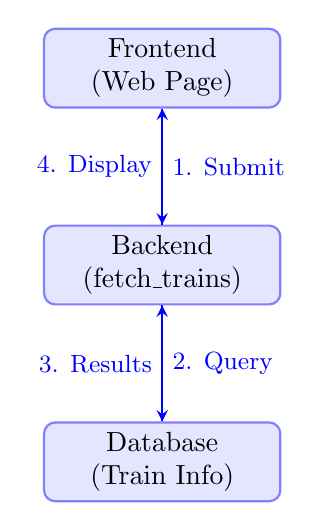
\begin{tikzpicture}[
    node distance=2.5cm,
    component/.style={rectangle, rounded corners, draw=blue!50, fill=blue!10, thick, minimum width=3cm, minimum height=1cm, align=center},
    arrow/.style={->, >=stealth, thick, blue}
]

% Nodes
\node[component] (frontend) {Frontend\\(Web Page)};
\node[component, below of=frontend] (backend) {Backend\\(fetch\_trains)};
\node[component, below of=backend] (database) {Database\\(Train Info)};

% Arrows
\draw[arrow] (frontend) -- node[right, font=\small] {1. Submit} (backend);
\draw[arrow] (backend) -- node[right, font=\small] {2. Query} (database);
\draw[arrow] (database) -- node[left, font=\small] {3. Results} (backend);
\draw[arrow] (backend) -- node[left, font=\small] {4. Display} (frontend);

\end{tikzpicture}
\end{center}

\textbf{Process:}
\begin{enumerate}[leftmargin=*]
    \item User submits form (Frontend)
    \item HTTP request calls \texttt{fetch\_trains()} function (Backend)
    \item Function queries Database
    \item Database returns information
    \item Results sent back to Frontend
    \item Frontend displays results to user
\end{enumerate}

\subsection{The Monolithic Architecture}

\begin{infobox}{What is Monolithic Architecture?}
An architecture where:
\begin{itemize}[leftmargin=*]
    \item All code exists in a single folder/directory
    \item Frontend and Backend in same application
    \item Both developed within one project structure
    \item Tightly coupled components
    \item Everything bundled as one application
\end{itemize}
\end{infobox}

\subsubsection{Key Characteristics}

\hspace{1.5em}\textbf{Single Application Structure:}
\begin{itemize}[leftmargin=*]
    \item One folder/directory contains everything
    \item Frontend code in same location as Backend code
    \item No separation between components
    \item Deployed as single unit
\end{itemize}

\textbf{Tightly Coupled:}
\begin{itemize}[leftmargin=*]
    \item Frontend directly connected to Backend
    \item No intermediary layer needed
    \item Can communicate without API
    \item Changes in one affect the other
\end{itemize}

\begin{notebox}
\textbf{Important Observation:}

\vspace{0.5em}
Notice that Backend and Frontend are communicating \textit{without an API}. This is possible because they're tightly coupled within the same application. They're not separate software components.
\end{notebox}

\subsubsection{Pre-API Website Development}

Before APIs:
\begin{itemize}[leftmargin=*]
    \item All websites used Monolithic Architecture
    \item Frontend and Backend weren't separate software pieces
    \item They were parts of one unified software
    \item This architecture was called "Monolithic"
\end{itemize}

\begin{warningbox}
\textbf{Technology Context:}

\vspace{0.5em}
For those familiar with PHP or Flask:
\begin{itemize}[leftmargin=*]
    \item If you've done web development with PHP (handling HTML files)
    \item Or used Flask to render HTML templates
    \item You've experienced Monolithic Architecture
    \item This is exactly what we're describing
\end{itemize}
\end{warningbox}

\subsection{The Problem with Monolithic Architecture}

\subsubsection{Initial Success}

\textbf{Good News:}
\begin{itemize}[leftmargin=*]
    \item IRCTC website built and working
    \item Using Monolithic Architecture
    \item Website functioning properly
    \item Users can search for trains successfully
\end{itemize}

\subsubsection{The Business Opportunity}

\textbf{New Development:}

\vspace{0.5em}
Several companies approach IRCTC:
\begin{itemize}[leftmargin=*]
    \item \textbf{MakeMyTrip}: Travel booking platform
    \item \textbf{Yatra}: Travel services company
    \item \textbf{Ixigo}: Travel search engine
\end{itemize}

\textbf{Their Request:}
\begin{itemize}[leftmargin=*]
    \item "Users ask us about train schedules too"
    \item "We don't have this information"
    \item "Only IRCTC has official railway data"
    \item "Can you give us access to this information?"
    \item "We'll pay per request"
\end{itemize}

\textbf{IRCTC's Perspective:}
\begin{itemize}[leftmargin=*]
    \item Great business opportunity
    \item Already providing data to our own users
    \item Other websites need it too
    \item Can earn money by sharing data
    \item Win-win situation
\end{itemize}

\subsubsection{The Technical Challenge}

\hspace{1.5em}\textbf{The Problem:}

\vspace{0.5em}

How to technically implement this data sharing?

\vspace{0.5em}
\textbf{What Needs to Happen:}
\begin{itemize}[leftmargin=*]
    \item MakeMyTrip, Yatra, and Ixigo need access to database information
    \item They are external software applications
    \item Need to access IRCTC's train schedule data
\end{itemize}

\textbf{Option 1: Direct Database Access}

\begin{warningbox}
\textbf{Why This Won't Work:}
\begin{itemize}[leftmargin=*]
    \item \textbf{Security Risk:} Cannot give direct database access to external companies
    \item \textbf{Data Integrity:} What if they accidentally modify data?
    \item \textbf{Control Loss:} No control over how they use the database
    \item \textbf{Not Feasible:} Too dangerous for production systems
\end{itemize}
\end{warningbox}

\textbf{Option 2: Backend Access}

\vspace{0.5em}

Remember our Backend has the \texttt{fetch\_trains()} function:
\begin{itemize}[leftmargin=*]
    \item Give two stations and a date
    \item Returns trains between those stations
    \item Seems like a safer option
\end{itemize}

\textbf{Ideal Scenario:}
\begin{itemize}[leftmargin=*]
    \item MakeMyTrip software interacts with Backend component
    \item MakeMyTrip sends: Station names + Date
    \item Backend receives and processes request
    \item Backend queries Database
    \item Backend returns response to MakeMyTrip
    \item MakeMyTrip displays to their users
\end{itemize}

\textbf{Same Process for Others:}
\begin{itemize}[leftmargin=*]
    \item Yatra can do the same
    \item Ixigo can do the same
    \item Seems like the solution!
\end{itemize}

\subsubsection{Why This Also Won't Work}

\begin{warningbox}
\textbf{The Fundamental Problem:}

\vspace{0.5em}
The Backend is \textit{not an independent application}. It's tightly coupled with the entire application.

\vspace{0.5em}
\textbf{Consequences:}
\begin{itemize}[leftmargin=*]
    \item Backend is part of Monolithic application
    \item Backend is one small component of larger software
    \item Backend is tightly coupled with other components
    \item Cannot be accessed independently from outside
    \item External software cannot interact with it directly
\end{itemize}
\end{warningbox}

\subsection{The Dead End}

\begin{center}
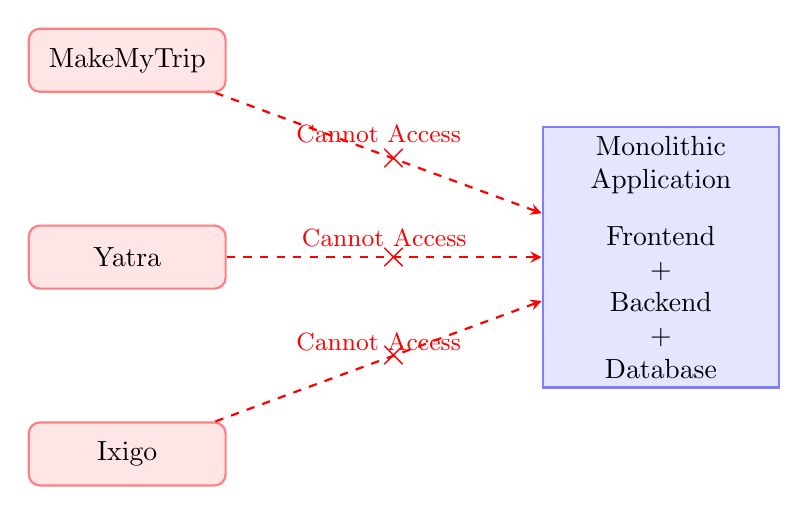
\begin{tikzpicture}[
    node distance=2.5cm,
    company/.style={rectangle, rounded corners, draw=red!50, fill=red!10, thick, minimum width=2.5cm, minimum height=0.8cm, align=center},
    system/.style={rectangle, draw=blue!50, fill=blue!10, thick, minimum width=3cm, minimum height=3cm, align=center},
    arrow/.style={->, >=stealth, thick, red, dashed}
]

% External companies
\node[company] (mmt) {MakeMyTrip};
\node[company, below of=mmt] (yatra) {Yatra};
\node[company, below of=yatra] (ixigo) {Ixigo};

% Monolithic system
\node[system, right=4cm of yatra] (mono) {Monolithic\\Application\\[0.3cm]Frontend\\+\\Backend\\+\\Database};

% Crossed out arrows
\draw[arrow] (mmt) -- node[above, font=\small] {Cannot Access} (mono);
\draw[arrow] (yatra) -- node[above, font=\small] {Cannot Access} (mono);
\draw[arrow] (ixigo) -- node[above, font=\small] {Cannot Access} (mono);

% X marks
\node[red, font=\Large] at ($(mmt)!0.5!(mono)$) {$\wrongmark$};
\node[red, font=\Large] at ($(yatra)!0.5!(mono)$) {$\wrongmark$};
\node[red, font=\Large] at ($(ixigo)!0.5!(mono)$) {$\wrongmark$};

\end{tikzpicture}
\end{center}

\textbf{Summary of the Problem:}

\begin{itemize}[leftmargin=*]
    \item Cannot share Database directly (security risk)
    \item Cannot share Backend directly (tightly coupled)
    \item Cannot provide access to internal information
    \item External software cannot interact with monolithic system
    \item Information is locked inside the monolithic application
\end{itemize}

\begin{infobox}{The Real Restriction}
The information in the database is ONLY shareable within your own Monolithic application. External parties cannot access it. This is a huge business limitation.

\vspace{0.5em}
\textbf{Business Impact:}
\begin{itemize}[leftmargin=*]
    \item IRCTC could earn money from other companies
    \item But the website architecture prevents it
    \item Massive revenue opportunity lost
    \item All because of technical limitations
\end{itemize}
\end{infobox}

\begin{warningbox}
\textbf{This is precisely the problem that APIs solve.}

\vspace{0.5em}
The inability to share data and functionality with external applications is the exact issue that necessitated the invention of APIs.
\end{warningbox}

\newpage

% ========================
% SECTION 4: API SOLUTION
% ========================
\section{The API Solution: Decoupled Architecture}

\subsection{Solving the Problem with APIs}

Now let's see how APIs solve the problems we identified with Monolithic Architecture.

\subsubsection{Step 1: Decoupling Backend from Frontend}

\textbf{The First Major Change:}

\vspace{0.5em}
Stop using Monolithic Architecture and decouple the application components.

\begin{infobox}{Decoupling Means:}
\begin{itemize}[leftmargin=*]
    \item Backend built separately
    \item Frontend built separately
    \item Backend = Different software application
    \item Frontend = Different software application
    \item No longer tightly coupled
\end{itemize}
\end{infobox}

\textbf{New Architecture Components:}

\begin{enumerate}[leftmargin=*]
    \item \textbf{Database}
    \begin{itemize}
        \item Still exists as before
        \item Contains all train information
        \item Same data, same structure
    \end{itemize}
    
    \item \textbf{Backend (Now Independent)}
    \begin{itemize}
        \item Separate software application
        \item Contains \texttt{fetch\_trains()} function
        \item Can query database independently
        \item Not connected to Frontend
        \item Standalone application
    \end{itemize}
    
    \item \textbf{API Layer (NEW)}
    \begin{itemize}
        \item Added in front of Backend
        \item Makes Backend publicly accessible
        \item Sits between Backend and Internet
        \item Gateway to Backend functionality
    \end{itemize}
    
    \item \textbf{Frontend (Now Independent)}
    \begin{itemize}
        \item Separate software application
        \item No direct connection to Backend
        \item Communicates through API
        \item Same user interface
    \end{itemize}
\end{enumerate}

\subsubsection{Step 2: Understanding the API Layer}

\begin{infobox}{What is an API Layer?}
An API is essentially a \textbf{set of endpoints}.

\vspace{0.5em}
\textbf{What are Endpoints?}
\begin{itemize}[leftmargin=*]
    \item Special types of functions
    \item Publicly available on the Internet
    \item Anyone can access them
    \item Have unique URLs
    \item Can be called/hit by anyone
\end{itemize}
\end{infobox}

\textbf{Example Endpoint:}

\begin{examplebox}{API Endpoint Example}
\textbf{Endpoint Name:} \texttt{/trains}

\vspace{0.5em}
\textbf{Characteristics:}
\begin{itemize}[leftmargin=*]
    \item It's a function (like any other function)
    \item But it's a \textit{special} function
    \item Available and present on the Internet
    \item Has a public URL
    \item Anyone can access it
\end{itemize}

\textbf{URL Example:}
\begin{verbatim}
https://irctc.com/api/trains
\end{verbatim}

\textbf{What it does:}
\begin{itemize}[leftmargin=*]
    \item When someone hits this URL
    \item Behind the scenes, it calls Backend's \texttt{fetch\_trains()} function
    \item Backend function queries Database
    \item Results returned through API
\end{itemize}
\end{examplebox}

\newpage

\subsection{The Complete API-Based Flow}

\subsubsection{Visual Representation}

\begin{center}
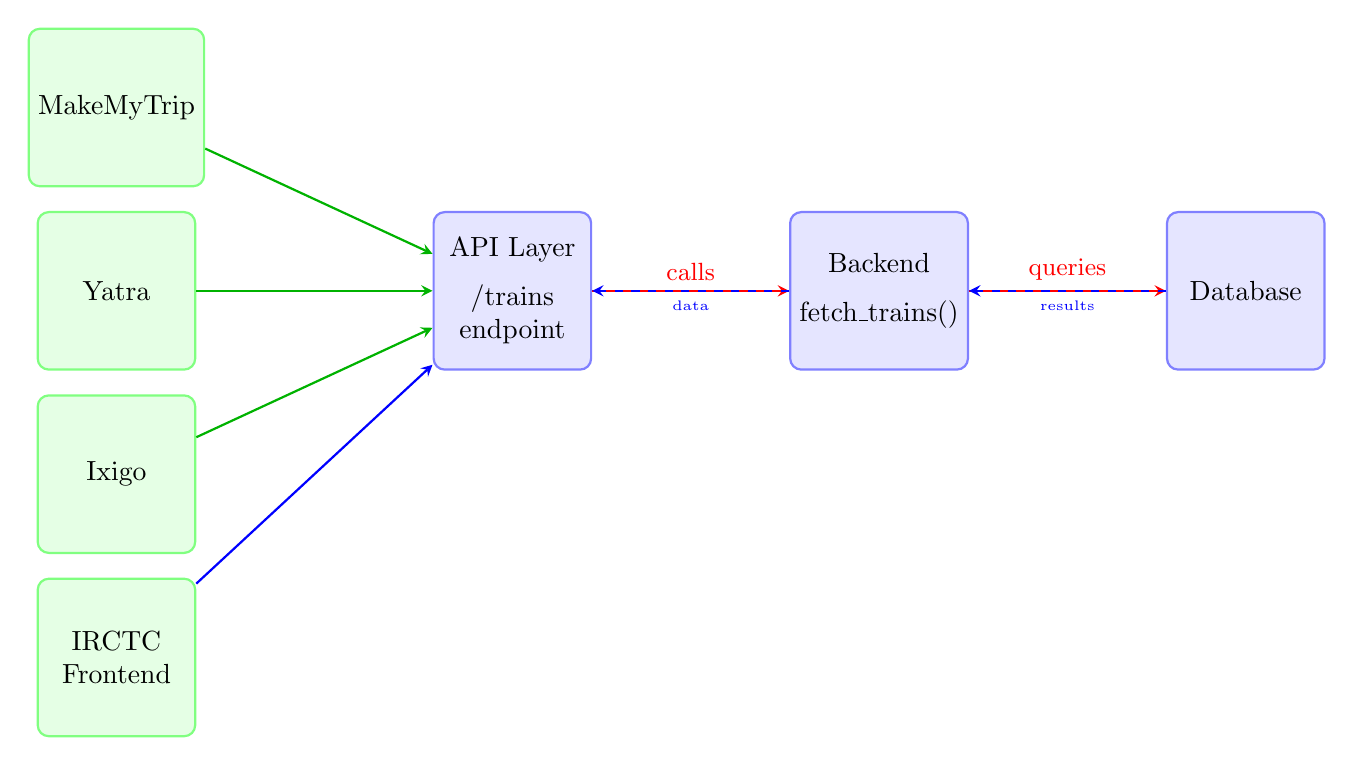
\begin{tikzpicture}[
    node distance=1cm,
    component/.style={rectangle, rounded corners, draw=blue!50, fill=blue!10, thick, minimum width=2cm, minimum height=2cm, align=center},
    client/.style={rectangle, rounded corners, draw=green!50, fill=green!10, thick, minimum width=2cm, minimum height=2cm, align=center},
    arrow/.style={->, >=stealth, thick}
]

% Clients
\node[client] (mmt) {MakeMyTrip};
\node[client, below=0.3cm of mmt] (yatra) {Yatra};
\node[client, below=0.3cm of yatra] (ixigo) {Ixigo};
\node[client, below=0.3cm of ixigo] (frontend) {IRCTC\\Frontend};

% API Layer
\node[component, right=3cm of yatra] (api) {API Layer\\[0.2cm]/trains\\endpoint};

% Backend
\node[component, right=2.5cm of api] (backend) {Backend\\[0.2cm]fetch\_trains()};

% Database
\node[component, right=2.5cm of backend] (db) {Database};

% Arrows from clients to API
\draw[arrow, green!70!black] (mmt) -- (api);
\draw[arrow, green!70!black] (yatra) -- (api);
\draw[arrow, green!70!black] (ixigo) -- (api);
\draw[arrow, blue] (frontend) -- (api);

% Arrows from API to Backend to Database
\draw[arrow, red] (api) -- node[above, font=\small] {calls} (backend);
\draw[arrow, red] (backend) -- node[above, font=\small] {queries} (db);

% Return arrows
\draw[arrow, blue, dashed] (db) -- node[below, font=\tiny] {results} (backend);
\draw[arrow, blue, dashed] (backend) -- node[below, font=\tiny] {data} (api);

\end{tikzpicture}
\end{center}

\subsubsection{Step-by-Step Process}

\textbf{Request Flow:}

\begin{enumerate}[leftmargin=*]
    \item \textbf{External Application Makes Request:}
    \begin{itemize}
        \item MakeMyTrip/Yatra/Ixigo hits API endpoint
        \item URL: \texttt{https://irctc.com/api/trains}
        \item Provides: Station1, Station2, Date
    \end{itemize}
    
    \item \textbf{API Receives Request:}
    \begin{itemize}
        \item API endpoint receives the request
        \item Extracts station names and date
        \item Prepares to call Backend
    \end{itemize}
    
    \item \textbf{API Calls Backend:}
    \begin{itemize}
        \item API invokes \texttt{fetch\_trains()} function
        \item Passes station names and date
        \item Backend function executes
    \end{itemize}
    
    \item \textbf{Backend Queries Database:}
    \begin{itemize}
        \item Backend searches for trains
        \item Finds trains between stations on given date
        \item Retrieves results from Database
    \end{itemize}
    
    \item \textbf{Results Return Path:}
    \begin{itemize}
        \item Database returns data to Backend
        \item Backend sends data to API
        \item API formats response (JSON)
        \item API sends response to requester
    \end{itemize}
    
    \item \textbf{Client Receives Response:}
    \begin{itemize}
        \item MakeMyTrip/Yatra/Ixigo receives data
        \item Displays information to their users
        \item Mission accomplished!
    \end{itemize}
\end{enumerate}

\subsection{Key Changes Made}

\begin{infobox}{Two Major Changes}
To solve the Monolithic Architecture problem:

\vspace{0.5em}
\textbf{Change 1: Decoupling}
\begin{itemize}[leftmargin=*]
    \item Separated Backend from Frontend
    \item Backend = Independent application
    \item Frontend = Independent application
    \item No tight coupling
\end{itemize}

\textbf{Change 2: API Layer}
\begin{itemize}[leftmargin=*]
    \item Added API layer in front of Backend
    \item Made Backend publicly accessible via Internet
    \item Backend available through API endpoints
    \item Anyone can access through proper API calls
\end{itemize}
\end{infobox}

\subsection{Benefits of API Architecture}

\subsubsection{Problem Solved}

\textbf{External Access:}
\begin{itemize}[leftmargin=*]
    \item Companies can now access IRCTC's data
    \item No direct database access (secure)
    \item No direct backend access (controlled)
    \item Access through API (safe and monitored)
\end{itemize}

\textbf{Revenue Generation:}
\begin{itemize}[leftmargin=*]
    \item IRCTC can charge per API request
    \item MakeMyTrip pays for each query
    \item Yatra pays for each query
    \item Ixigo pays for each query
    \item New business model enabled
\end{itemize}

\subsubsection{Additional Advantages}

\textbf{Security and Control:}
\begin{itemize}[leftmargin=*]
    \item API can implement security checks
    \item Validate incoming requests
    \item Prevent malicious data
    \item Authentication and authorization
    \item Rate limiting
    \item Logging and monitoring
\end{itemize}

\begin{examplebox}{API Security Example}
\begin{lstlisting}[language=Python]
# API endpoint can validate requests
def trains_endpoint(station1, station2, date):
    # Security checks
    if not is_valid_station(station1):
        return error("Invalid station")
    
    if not is_valid_date(date):
        return error("Invalid date")
    
    # Check API key/authentication
    if not is_authenticated():
        return error("Unauthorized")
    
    # Only then call backend
    result = backend.fetch_trains(station1, station2, date)
    return format_as_json(result)
\end{lstlisting}
\end{examplebox}

\textbf{IRCTC's Own Frontend:}

\vspace{0.5em}

Important note: IRCTC's own Frontend is NOT special!

\begin{itemize}[leftmargin=*]
    \item IRCTC Frontend is now a separate application
    \item It also uses the same API
    \item Same treatment as MakeMyTrip/Yatra/Ixigo
    \item Goes through API to reach Backend
    \item No direct Backend access
\end{itemize}

\begin{notebox}
\textbf{Key Insight:}

\vspace{0.5em}
The API-based architecture treats all clients equally:
\begin{itemize}[leftmargin=*]
    \item Your own Frontend
    \item External companies
    \item Mobile apps
    \item Third-party services
\end{itemize}

Everyone goes through the API. This ensures consistency, security, and scalability.
\end{notebox}

\subsection{Making Database Knowledge Available to All}

\textbf{The Big Picture:}

\begin{itemize}[leftmargin=*]
    \item Database information is now accessible to everyone
    \item Not directly, but through controlled API access
    \item IRCTC can share data safely
    \item External parties can use the data
    \item IRCTC generates revenue
    \item Win-win for all stakeholders
\end{itemize}

\begin{infobox}{Business Impact}
\textbf{Before API:}
\begin{itemize}[leftmargin=*]
    \item Data locked in monolithic system
    \item No way to share with external parties
    \item Lost revenue opportunities
    \item Limited ecosystem
\end{itemize}

\textbf{After API:}
\begin{itemize}[leftmargin=*]
    \item Data accessible through controlled endpoints
    \item External companies can integrate
    \item Revenue generation through API access
    \item Thriving ecosystem
\end{itemize}
\end{infobox}

\newpage

% ========================
% SECTION 5: PROTOCOLS AND DATA FORMATS
% ========================
\section{API Protocols and Data Formats}

\subsection{Revisiting the Definition}

Let's look again at the API definition with deeper understanding:

\begin{infobox}{API Definition - Revisited}
\textbf{APIs are mechanisms that enable two software components (such as the frontend and backend of an application) to communicate with each other using a defined set of rules, protocols, and data formats.}
\end{infobox}

Now we understand:
\begin{itemize}[leftmargin=*]
    \item ✓ How API acts as a connector
    \item ✓ How it connects two software components
    \item → Now let's understand: Protocols and Data Formats
\end{itemize}

\subsection{Protocols in API Communication}

\subsubsection{What is HTTP Protocol?}

When communicating over the Internet:
\begin{itemize}[leftmargin=*]
    \item All web-based communication uses \textbf{HTTP protocol}
    \item HTTP = HyperText Transfer Protocol
    \item Standard protocol for web applications
    \item Defines how requests and responses are formatted
\end{itemize}

\begin{examplebox}{HTTP in Our Example}
In the IRCTC example:
\begin{itemize}[leftmargin=*]
    \item MakeMyTrip sends request to API: Uses HTTP
    \item API communicates with Backend: Uses HTTP
    \item Backend returns response: Uses HTTP
    \item Response sent to MakeMyTrip: Uses HTTP
\end{itemize}

Everything happening over the Internet follows HTTP protocol.
\end{examplebox}

\subsection{Data Formats: JSON}

\subsubsection{The Need for Universal Format}

\textbf{The Challenge:}

\vspace{0.5em}
Consider our API clients:
\begin{itemize}[leftmargin=*]
    \item MakeMyTrip might be built in \textbf{Java}
    \item Yatra might be built in \textbf{Python}
    \item Ixigo might be built in \textbf{PHP}
\end{itemize}

\textbf{The Question:}

\vspace{0.5em}
When API returns response, what format should it use?
\begin{itemize}[leftmargin=*]
    \item Java needs to understand it
    \item Python needs to understand it
    \item PHP needs to understand it
    \item Need a universal format!
\end{itemize}

\subsubsection{JSON: The Universal Data Format}

\begin{infobox}{JSON - JavaScript Object Notation}
\textbf{What is JSON?}
\begin{itemize}[leftmargin=*]
    \item Universal data format
    \item Language-independent
    \item Human-readable
    \item Machine-parseable
    \item Industry standard for APIs
\end{itemize}

\textbf{Why JSON?}
\begin{itemize}[leftmargin=*]
    \item Java can understand JSON
    \item Python can understand JSON
    \item PHP can understand JSON
    \item Every programming language supports JSON
    \item Perfect for API responses
\end{itemize}
\end{infobox}

\subsubsection{JSON Format Example}

\begin{examplebox}{JSON Response Example}
\begin{lstlisting}[language=Python]
# API returns data in JSON format
{
    "trains": [
        {
            "train_number": "12345",
            "train_name": "Rajdhani Express",
            "departure": "10:00 AM",
            "arrival": "08:00 PM"
        },
        {
            "train_number": "12346",
            "train_name": "Shatabdi Express",
            "departure": "02:00 PM",
            "arrival": "10:00 PM"
        }
    ],
    "status": "success",
    "count": 2
}
\end{lstlisting}
\end{examplebox}

\begin{notebox}
\textbf{For Python Developers:}

\vspace{0.5em}
If you've worked with Python dictionaries, JSON looks very similar!

\begin{lstlisting}[language=Python]
# Python dictionary
data = {
    "name": "John",
    "age": 30,
    "city": "New York"
}

# Almost identical to JSON!
\end{lstlisting}

We'll see JSON formatting in detail when we write code in FastAPI.
\end{notebox}

\subsection{Key Takeaways}

\begin{infobox}{Three Important Points}
\textbf{1. API as Connector:}
\begin{itemize}[leftmargin=*]
    \item Connects two software components
    \item In our case: IRCTC Backend <-> External Applications
\end{itemize}

\textbf{2. Protocol - HTTP:}
\begin{itemize}[leftmargin=*]
    \item Communication follows HTTP protocol
    \item Standard for Internet-based communication
\end{itemize}

\textbf{3. Data Format - JSON:}
\begin{itemize}[leftmargin=*]
    \item Responses returned in JSON format
    \item Universal format understood by all languages
    \item Client can be in any language - no problem!
\end{itemize}
\end{infobox}

\newpage

% ========================
% SECTION 6: THE SECOND PROBLEM
% ========================
\section{The Second Problem: Multiple Platforms}

\subsection{The Smartphone Revolution}

\subsubsection{The Timeline: 2008-2012}

\hspace{1.5em}\textbf{Before 2008:}
\begin{itemize}[leftmargin=*]
    \item Nobody had smartphones
    \item Only basic mobile phones existed
    \item Desktop/laptop was primary way to access internet
\end{itemize}

\textbf{2008-2012:}
\begin{itemize}[leftmargin=*]
    \item Smartphone revolution began
    \item By 2012, most people had smartphones
    \item Two major categories emerged:
    \begin{itemize}
        \item Android phones
        \item iPhones (iOS)
    \end{itemize}
\end{itemize}

\subsection{The Multi-Platform Challenge}

\subsubsection{Business Realization}

Companies started realizing:
\begin{itemize}[leftmargin=*]
    \item Just a website isn't enough
    \item To expand business opportunities
    \item Need to be on multiple platforms
    \item Should build:
    \begin{itemize}
        \item Website (for desktop users)
        \item Android app (for Android users)
        \item iPhone app (for iOS users)
    \end{itemize}
\end{itemize}

\textbf{The Goal:}
\begin{itemize}[leftmargin=*]
    \item Provide seamless connectivity to users
    \item Users can access application from any platform
    \item Same functionality across all platforms
    \item Better user experience
    \item Increased user base
\end{itemize}

\subsubsection{Current Reality (2025)}

\begin{examplebox}{Multi-Platform Reality}
Pick any application today:
\begin{itemize}[leftmargin=*]
    \item Most likely has a website
    \item Most likely has an Android app
    \item Most likely has an iPhone app
\end{itemize}

Examples:
\begin{itemize}[leftmargin=*]
    \item Social media: Instagram, Facebook, Twitter
    \item E-commerce: Amazon, Flipkart
    \item Food delivery: Zomato, Swiggy
    \item Ride sharing: Uber, Ola
    \item Entertainment: Netflix, Spotify
\end{itemize}

All available on Web + Android + iOS
\end{examplebox}

\subsection{The Technical Challenge}

\subsubsection{Different Technology Stacks}

\textbf{The Problem:}

\vspace{0.5em}
Each platform requires different technology:

\begin{center}
\begin{tabular}{|l|l|l|}
\hline
\textbf{Platform} & \textbf{Language} & \textbf{Tech Stack} \\
\hline
Website & JavaScript/Python/PHP & HTML, CSS, JS \\
\hline
Android App & Java/Kotlin & Android SDK \\
\hline
iPhone App & Swift/Objective-C & iOS SDK \\
\hline
\end{tabular}
\end{center}

\textbf{What This Means:}
\begin{itemize}[leftmargin=*]
    \item Completely different tech stack for Android
    \item Completely different tech stack for iOS
    \item Completely different tech stack for Web
    \item Cannot reuse code across platforms
\end{itemize}

\subsubsection{The Monolithic Approach Problem}

\textbf{If Using Monolithic Architecture:}

\vspace{0.5em}
Would need to build:
\begin{enumerate}[leftmargin=*]
    \item One Monolithic application for Website
    \item One Monolithic application for Android app
    \item One Monolithic application for iPhone app
\end{enumerate}

\textbf{Consequences:}

\begin{warningbox}
\textbf{Major Problems with Three Monolithic Apps:}

\vspace{0.5em}
\textbf{Problem 1: Independence}
\begin{itemize}[leftmargin=*]
    \item All three applications are independent
    \item Changes must be made to all three
    \item User comments on website? Must update Android and iOS
    \item User uploads photo on Android? Must sync to Web and iOS
    \item Everything needs to be synchronized manually
\end{itemize}

\textbf{Problem 2: Team Requirements}
\begin{itemize}[leftmargin=*]
    \item Need three separate development teams
    \item Web development team
    \item Android development team
    \item iOS development team
    \item Significant additional cost
\end{itemize}

\textbf{Problem 3: Maintenance Nightmare}
\begin{itemize}[leftmargin=*]
    \item Three codebases to maintain
    \item Three sets of bugs to fix
    \item Three deployments for every feature
    \item Extremely difficult to keep synchronized
\end{itemize}
\end{warningbox}

\subsection{The API-Based Solution}

\subsubsection{The Elegant Architecture}

Instead of three Monolithic applications, use API architecture:

\begin{infobox}{API-Based Multi-Platform Architecture}
\textbf{Single Backend + Multiple Frontends}

\vspace{0.5em}
\textbf{Backend (One):}
\begin{itemize}[leftmargin=*]
    \item One Database (single source of truth)
    \item One Backend application
    \item One API layer
    \item Handles all business logic
\end{itemize}

\textbf{Frontends (Multiple):}
\begin{itemize}[leftmargin=*]
    \item Website Frontend (separate)
    \item Android App Frontend (separate)
    \item iOS App Frontend (separate)
    \item All connect to same API
\end{itemize}
\end{infobox}

\subsubsection{Visual Architecture}

\begin{center}
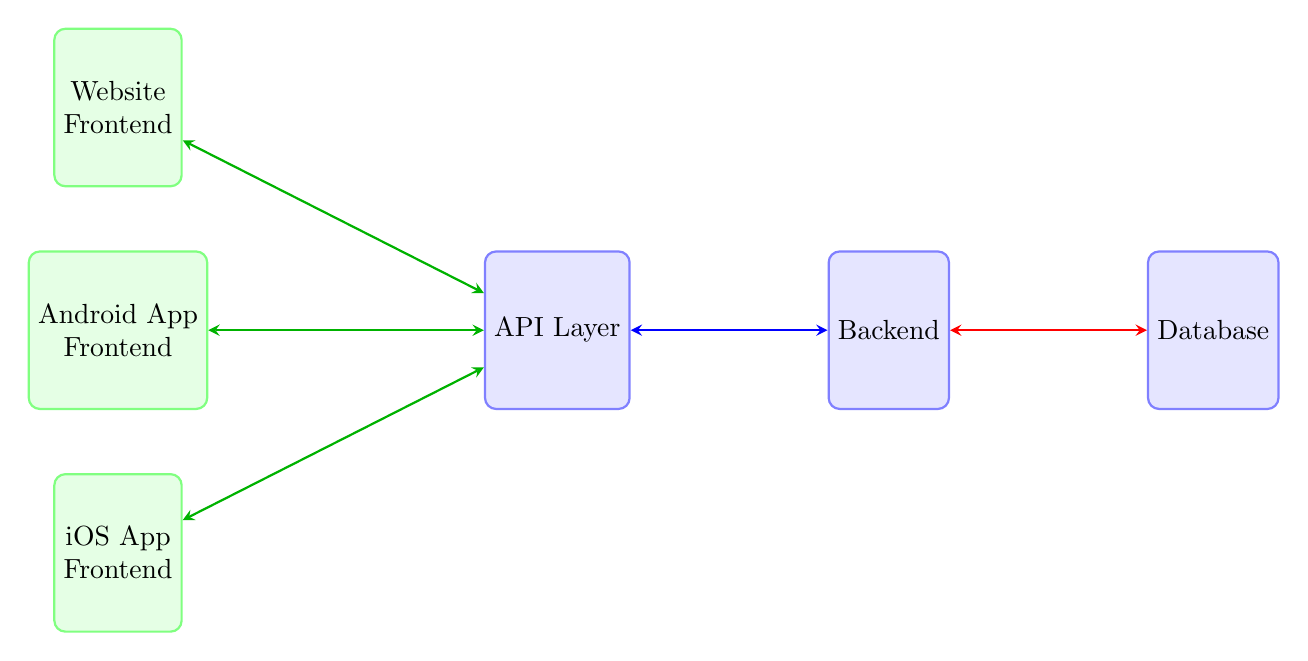
\begin{tikzpicture}[
    node distance=1.5cm,
    frontend/.style={rectangle, rounded corners, draw=green!50, fill=green!10, thick, minimum width=1.5cm, minimum height=2cm, align=center},
    backend/.style={rectangle, rounded corners, draw=blue!50, fill=blue!10, thick, minimum width=1.5cm, minimum height=2cm, align=center},
    arrow/.style={<->, >=stealth, thick}
]

% Frontends
\node[frontend] (web) {Website\\Frontend};
\node[frontend, below=0.8cm of web] (android) {Android App\\Frontend};
\node[frontend, below=0.8cm of android] (ios) {iOS App\\Frontend};

% API Layer
\node[backend, right=3.5cm of android] (api) {API Layer};

% Backend
\node[backend, right=2.5cm of api] (backend) {Backend};

% Database
\node[backend, right=2.5cm of backend] (db) {Database};

% Arrows
\draw[arrow, green!70!black] (web) -- (api);
\draw[arrow, green!70!black] (android) -- (api);
\draw[arrow, green!70!black] (ios) -- (api);
\draw[arrow, blue] (api) -- (backend);
\draw[arrow, red] (backend) -- (db);

\end{tikzpicture}
\end{center}

\subsubsection{How It Works}

\textbf{The Flow:}

\begin{enumerate}[leftmargin=*]
    \item \textbf{User Makes Request:}
    \begin{itemize}
        \item Could be from Website, Android, or iOS
        \item Request goes to API
    \end{itemize}
    
    \item \textbf{API Processes:}
    \begin{itemize}
        \item API receives request
        \item Forwards to Backend
        \item Doesn't care which frontend sent it
    \end{itemize}
    
    \item \textbf{Backend Processes:}
    \begin{itemize}
        \item Backend handles business logic
        \item Queries Database if needed
        \item Processes data
    \end{itemize}
    
    \item \textbf{Response Returns:}
    \begin{itemize}
        \item Database → Backend → API
        \item API formats as JSON
        \item JSON sent to requesting frontend
    \end{itemize}
    
    \item \textbf{Frontend Displays:}
    \begin{itemize}
        \item Each frontend displays in its own way
        \item Website: HTML/CSS rendering
        \item Android: Native Android UI
        \item iOS: Native iOS UI
    \end{itemize}
\end{enumerate}

\subsection{Benefits of API-Based Multi-Platform}

\subsubsection{Simplified Architecture}

\begin{itemize}[leftmargin=*]
    \item \textbf{One Database}: Single source of truth for all data
    \item \textbf{One Backend}: All business logic in one place
    \item \textbf{One API}: Single gateway for all platforms
    \item \textbf{Multiple Frontends}: Platform-specific UIs only
\end{itemize}

\subsubsection{Development Benefits}

\hspace{1.5em}\textbf{No Need for Separate Backends:}
\begin{itemize}[leftmargin=*]
    \item Don't need three different backend implementations
    \item Same backend serves all platforms
    \item Write business logic once, use everywhere
\end{itemize}

\textbf{No Need for Multiple Databases:}
\begin{itemize}[leftmargin=*]
    \item Don't maintain three databases
    \item All data in one place
    \item Automatic synchronization
    \item Data consistency guaranteed
\end{itemize}

\textbf{Frontend Focus:}
\begin{itemize}[leftmargin=*]
    \item Frontend teams only worry about UI/UX
    \item Each platform optimized independently
    \item Same data, different presentation
\end{itemize}

\subsubsection{Real-World Examples}

\begin{examplebox}{Industry Implementation}
\textbf{Companies Using This Architecture:}

\vspace{0.5em}
\textbf{Google:}
\begin{itemize}[leftmargin=*]
    \item One backend API
    \item Multiple frontends: Web, Android, iOS, Desktop
    \item Same Gmail data everywhere
\end{itemize}

\textbf{Uber:}
\begin{itemize}[leftmargin=*]
    \item One backend system
    \item Passenger apps: Web, Android, iOS
    \item Driver apps: Android, iOS
    \item All hitting same APIs
\end{itemize}

\textbf{Zomato:}
\begin{itemize}[leftmargin=*]
    \item Single database of restaurants
    \item One backend with APIs
    \item Website + Android + iOS apps
    \item Consistent experience everywhere
\end{itemize}
\end{examplebox}

\begin{notebox}
Today, if you examine any major company (Google, Uber, Zomato, etc.), you'll find:
\begin{itemize}[leftmargin=*]
    \item Single database
    \item Backend connected to database
    \item Backend accessible via API
    \item Multiple frontends consuming the API
\end{itemize}

This is the standard architecture for modern applications.
\end{notebox}

\subsection{Summary: Two Problems Solved}

\begin{infobox}{Problem 1: External Access}
\textbf{Challenge:}
\begin{itemize}[leftmargin=*]
    \item External companies needed access to data
    \item Monolithic architecture prevented sharing
    \item No way to monetize data safely
\end{itemize}

\textbf{Solution:}
\begin{itemize}[leftmargin=*]
    \item Decouple Backend from Frontend
    \item Add API layer
    \item External parties access through API
    \item Secure, controlled access
    \item Revenue generation possible
\end{itemize}
\end{infobox}

\begin{infobox}{Problem 2: Multiple Platforms}
\textbf{Challenge:}
\begin{itemize}[leftmargin=*]
    \item Need Website, Android, and iOS apps
    \item Different tech stacks for each
    \item Maintaining three monolithic apps too complex
    \item Synchronization nightmare
\end{itemize}

\textbf{Solution:}
\begin{itemize}[leftmargin=*]
    \item Single Backend + API
    \item Multiple independent Frontends
    \item All Frontends use same API
    \item Simplified architecture
    \item Easy maintenance
    \item Automatic synchronization
\end{itemize}
\end{infobox}

\newpage

% ========================
% SECTION 7: APIs IN MACHINE LEARNING
% ========================
\section{APIs in Machine Learning Context}

\subsection{Software vs ML: The Key Difference}

Now let's understand how these API principles apply specifically to Machine Learning.

\subsubsection{The Core Difference}

\begin{center}
\begin{tabular}{|p{0.45\textwidth}|p{0.45\textwidth}|}
\hline
\textbf{Software Applications} & \textbf{ML Applications} \\
\hline
Most important: \textbf{Database} & Most important: \textbf{ML Model} \\
\hline
Data stored in database & Data learned by model \\
\hline
Query database for information & Query model for predictions \\
\hline
Backend interacts with database & Backend interacts with model \\
\hline
\end{tabular}
\end{center}

\begin{infobox}{Key Insight}
\textbf{In Machine Learning:}

\vspace{0.5em}
Replace "Database" with "ML Model" and the entire architecture remains the same!

\begin{itemize}[leftmargin=*]
    \item Database → ML Model
    \item Query → Prediction Request
    \item Results → Predictions
    \item Everything else identical
\end{itemize}
\end{infobox}

\subsection{ML Model Deployment Journey}

\subsubsection{The ML Development Process}

\begin{enumerate}[leftmargin=*]
    \item \textbf{Model Training:}
    \begin{itemize}
        \item Train model on large dataset
        \item Could be ML, DL, or Generative AI
        \item Iterate until good results
    \end{itemize}
    
    \item \textbf{Model Evaluation:}
    \begin{itemize}
        \item Model starts giving good results
        \item Metrics look promising
        \item Ready for production
    \end{itemize}
    
    \item \textbf{Deployment Decision:}
    \begin{itemize}
        \item Want to present model to world
        \item Need to monetize
        \item Build application around model
    \end{itemize}
    
    \item \textbf{Application Building:}
    \begin{itemize}
        \item Build around the model
        \item Create user interface
        \item Enable model access
    \end{itemize}
\end{enumerate}

\subsection{Case Study: ChatGPT}

Let's understand ML APIs through the world's most famous AI product.

\subsubsection{ChatGPT Background}

\hspace{1.5em}\textbf{What is ChatGPT?}
\begin{itemize}[leftmargin=*]
    \item Built by OpenAI
    \item Powered by GPT models (LLMs)
    \item Most famous AI product currently
    \item Uses Large Language Models
\end{itemize}

\textbf{OpenAI's Process:}
\begin{enumerate}[leftmargin=*]
    \item Trained GPT model on massive data
    \item Model started producing good results
    \item Decided to monetize the model
    \item Best way: Present it via a website
\end{enumerate}

\textbf{The Goal:}
\begin{itemize}[leftmargin=*]
    \item Users visit website
    \item Users ask questions
	\item Questions sent to GPT model
    \item Model generates responses
    \item Responses displayed to users
\end{itemize}

\subsection{Pre-API ML Application Architecture}

\subsubsection{The Monolithic ML Approach}

Before APIs, ML applications were built as monolithic systems:

\begin{center}
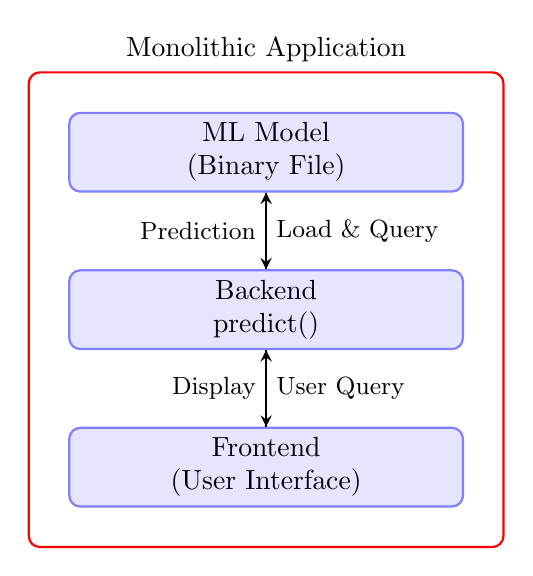
\begin{tikzpicture}[
    node distance=2cm,
    component/.style={rectangle, rounded corners, draw=blue!50, fill=blue!10, thick, minimum width=5cm, minimum height=1cm, align=center},
    arrow/.style={->, >=stealth, thick}
]

% Components
\node[component] (model) {ML Model\\(Binary File)};
\node[component, below of=model] (backend) {Backend\\predict()};
\node[component, below of=backend] (frontend) {Frontend\\(User Interface)};

% Arrows
\draw[arrow] (frontend) -- node[right, font=\small] {User Query} (backend);
\draw[arrow] (backend) -- node[right, font=\small] {Load \& Query} (model);
\draw[arrow] (model) -- node[left, font=\small] {Prediction} (backend);
\draw[arrow] (backend) -- node[left, font=\small] {Display} (frontend);

% Box around all
\node[draw=red, thick, rounded corners, fit=(model)(backend)(frontend), inner sep=0.5cm, label=above:Monolithic Application] {};

\end{tikzpicture}
\end{center}

\subsubsection{Components Breakdown}

\textbf{1. ML Model (Binary File):}
\begin{itemize}[leftmargin=*]
    \item Trained model saved as file
    \item Could be .pkl, .h5, .pth, etc.
    \item Not a database - it's a file
    \item Can be loaded in any programming language
\end{itemize}

\textbf{2. Backend:}
\begin{itemize}[leftmargin=*]
    \item Functions to interact with model
    \item \texttt{predict()} function example
    \item Takes user data
    \item Loads model
    \item Sends data to model
    \item Returns prediction
\end{itemize}

\begin{examplebox}{Backend Prediction Function}
\begin{lstlisting}[language=Python]
def predict(user_query):
    """
    Load ML model and get prediction
    """
    # Load the trained model
    model = load_model('chatbot_model.pkl')
    
    # Get prediction from model
    response = model.generate_response(user_query)
    
    # Return the response
    return response
\end{lstlisting}
\end{examplebox}

\vspace{0.5em}
\textbf{3. Frontend:}
\begin{itemize}[leftmargin=*]
    \item User interface
    \item Similar to ChatGPT interface
    \item Text input box for questions
    \item Submit button
    \item Display area for responses
\end{itemize}

\subsubsection{The Monolithic ML Flow}

\begin{enumerate}[leftmargin=*]
    \item \textbf{User Interaction:}
    \begin{itemize}
        \item User opens website (Frontend)
        \item Types question in text box
        \item Clicks Submit
    \end{itemize}
    
    \item \textbf{Request Processing:}
    \begin{itemize}
        \item User query sent to Backend
        \item \texttt{predict()} function called
        \item Function receives query
    \end{itemize}
    
    \item \textbf{Model Inference:}
    \begin{itemize}
        \item Backend loads ML model
        \item Sends query to model
        \item "What should the answer be?"
    \end{itemize}
    
    \item \textbf{Response Generation:}
    \begin{itemize}
        \item Model generates answer
        \item Based on its training
        \item Returns answer to Backend
    \end{itemize}
    
    \item \textbf{Display Result:}
    \begin{itemize}
        \item Backend sends answer to Frontend
        \item Frontend displays to user
        \item User sees the response
    \end{itemize}
\end{enumerate}

\subsubsection{The Problem with Monolithic ML Apps}

\begin{warningbox}
\textbf{Same Issues as Regular Applications:}

\vspace{0.5em}
\textbf{Tight Coupling:}
\begin{itemize}[leftmargin=*]
    \item Everything in one folder/application
    \item Frontend, Backend, Model all together
    \item One unified monolithic application
    \item Difficult to scale
    \item Difficult to maintain
\end{itemize}

\textbf{Cannot Share Model:}
\begin{itemize}[leftmargin=*]
    \item External applications cannot access
    \item Cannot monetize model separately
    \item Limited to own frontend only
    \item No ecosystem development
\end{itemize}
\end{warningbox}

\subsection{Real-World ML Business Scenario}

\subsubsection{The ChatGPT Opportunity}

When ChatGPT launched, many companies realized its potential:

\begin{examplebox}{Business Use Cases}
\textbf{1. Swiggy/Zomato - Food Delivery:}
\begin{itemize}[leftmargin=*]
    \item Use automated chatbots for customer service
    \item But chatbots weren't very good
    \item Poor responses, bad user experience
    \item Saw ChatGPT's capabilities
    \item Thought: "If we could use ChatGPT for our chatbot, user experience would improve dramatically"
\end{itemize}

\textbf{2. Amazon - E-commerce:}
\begin{itemize}[leftmargin=*]
    \item Thousands of product reviews
    \item Users don't read all reviews
    \item Thought: "What if we use GPT to summarize reviews?"
    \item Show users a condensed summary
    \item Improved shopping experience
\end{itemize}

\textbf{3. Document Analysis Companies:}
\begin{itemize}[leftmargin=*]
    \item Need question-answering on documents
    \item Thought: "What if we build RAG system with GPT?"
    \item Use GPT model for document Q\&A
    \item Better than traditional search
\end{itemize}
\end{examplebox}

\subsubsection{The Business Problem}

\textbf{The Desire:}

\vspace{0.5em}
Many companies want to use ChatGPT's capabilities:
\begin{itemize}[leftmargin=*]
    \item Chatbot improvements
    \item Review summarization
    \item Document Q\&A (RAG systems)
    \item Various other applications
\end{itemize}

\vspace{0.5em}
\textbf{The Blocker:}

\begin{warningbox}
\textbf{Cannot Access the Model:}

\vspace{0.5em}
Because OpenAI's application is Monolithic:
\begin{itemize}[leftmargin=*]
    \item Cannot directly access the GPT model
    \item Cannot directly access the Backend
    \item Model and Backend are tightly coupled
    \item No way for external apps to integrate
    \item Same problem we saw with IRCTC!
\end{itemize}
\end{warningbox}

\subsection{The API Solution for ML}

\subsubsection{Decoupling the ML Application}

The solution is identical to regular software - use APIs!

\begin{center}
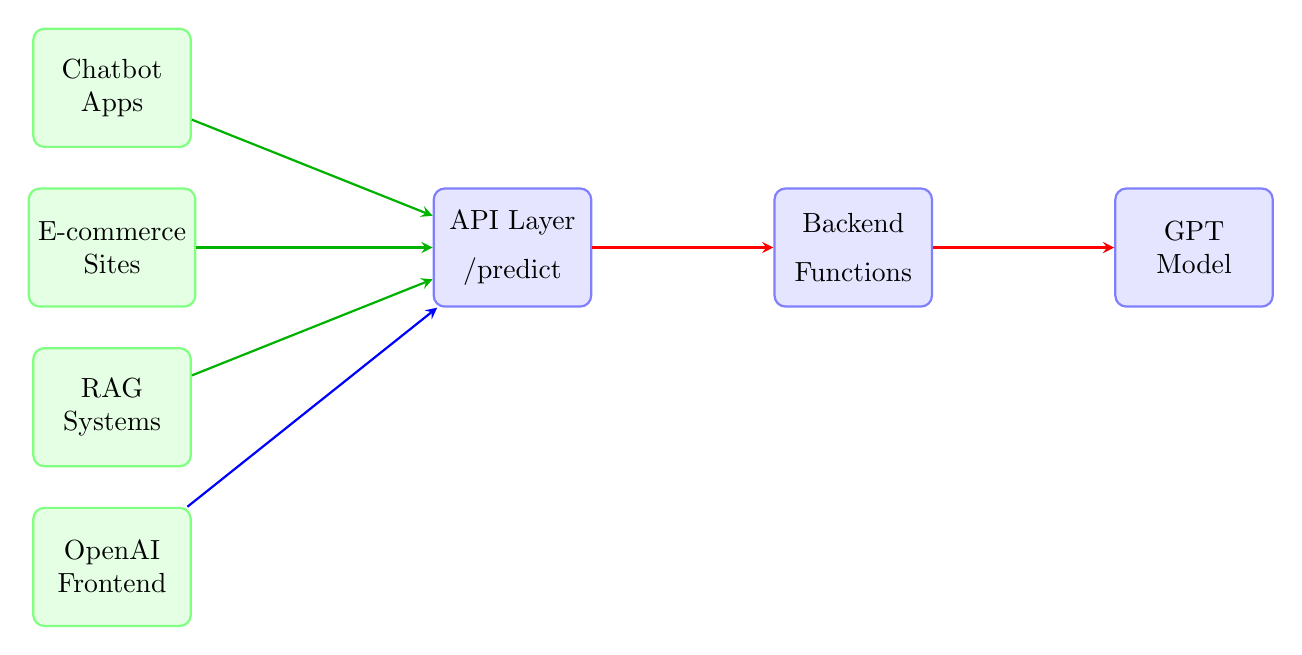
\begin{tikzpicture}[
    node distance=2cm,
    component/.style={rectangle, rounded corners, draw=blue!50, fill=blue!10, thick, minimum width=2cm, minimum height=1.5cm, align=center},
    client/.style={rectangle, rounded corners, draw=green!50, fill=green!10, thick, minimum width=2cm, minimum height=1.5cm, align=center},
    arrow/.style={->, >=stealth, thick}
]

% External clients
\node[client] (chatbot) {Chatbot\\Apps};
\node[client, below=0.5cm of chatbot] (ecom) {E-commerce\\Sites};
\node[client, below=0.5cm of ecom] (rag) {RAG\\Systems};
\node[client, below=0.5cm of rag] (frontend) {OpenAI\\Frontend};

% API Layer
\node[component, right=3cm of ecom] (api) {API Layer\\[0.2cm]/predict};

% Backend
\node[component, right=2.3cm of api] (backend) {Backend\\[0.2cm]Functions};

% ML Model
\node[component, right=2.3cm of backend] (model) {GPT\\Model};

% Arrows
\draw[arrow, green!70!black] (chatbot) -- (api);
\draw[arrow, green!70!black] (ecom) -- (api);
\draw[arrow, green!70!black] (rag) -- (api);
\draw[arrow, blue] (frontend) -- (api);
\draw[arrow, red] (api) -- (backend);
\draw[arrow, red] (backend) -- (model);

\end{tikzpicture}
\end{center}

\subsubsection{The New Architecture}

\textbf{Components:}

\begin{enumerate}[leftmargin=*]
    \item \textbf{ML Model (Independent):}
    \begin{itemize}
        \item GPT model as separate entity
        \item Saved as binary file
        \item Can be loaded and queried
    \end{itemize}
    
    \item \textbf{Backend (Independent):}
    \begin{itemize}
        \item Separate application
        \item Contains functions to interact with model
        \item Loads model and gets predictions
        \item Not connected to Frontend directly
    \end{itemize}
    
    \item \textbf{API Layer (Gateway):}
    \begin{itemize}
        \item Sits in front of Backend
        \item Makes Backend publicly accessible
        \item Endpoints available on Internet
        \item Anyone can hit these endpoints
    \end{itemize}
    
    \item \textbf{Frontend (Independent):}
    \begin{itemize}
        \item OpenAI's ChatGPT interface
        \item Separate application
        \item Communicates through API only
    \end{itemize}
    
    \item \textbf{External Applications:}
    \begin{itemize}
        \item Other companies' applications
        \item Chatbots, e-commerce sites, RAG systems
        \item All communicate through API
    \end{itemize}
\end{enumerate}

\subsubsection{Complete ML API Flow}

\begin{enumerate}[leftmargin=*]
    \item \textbf{External App Makes Request:}
    \begin{itemize}
        \item Zomato's chatbot needs a response
        \item Hits API endpoint with user query
        \item \texttt{POST /api/predict}
    \end{itemize}
    
    \item \textbf{API Receives Request:}
    \begin{itemize}
        \item API endpoint receives query
        \item Validates request
        \item Forwards to Backend
    \end{itemize}
    
    \item \textbf{Backend Processes:}
    \begin{itemize}
        \item Backend function called
        \item Loads GPT model
        \item Sends query to model
    \end{itemize}
    
    \item \textbf{Model Generates Response:}
    \begin{itemize}
        \item GPT model processes query
        \item Generates answer
        \item Returns to Backend
    \end{itemize}
    
    \item \textbf{Response Returns:}
    \begin{itemize}
        \item Backend sends response to API
        \item API formats as JSON
        \item JSON sent back to requester
    \end{itemize}
    
    \item \textbf{Client Uses Response:}
    \begin{itemize}
        \item Zomato's chatbot receives response
        \item Displays to their users
        \item Improved user experience!
    \end{itemize}
\end{enumerate}

\subsection{ML API Architecture Comparison}

\begin{center}
\begin{tabular}{|p{0.45\textwidth}|p{0.45\textwidth}|}
\hline
\textbf{Software APIs} & \textbf{ML APIs} \\
\hline
Database stores data & ML Model stores learned patterns \\
\hline
Backend queries database & Backend queries model \\
\hline
Returns data results & Returns predictions \\
\hline
API exposes data access & API exposes prediction access \\
\hline
HTTP protocol & HTTP protocol \\
\hline
JSON data format & JSON data format \\
\hline
Multiple frontends access & Multiple apps access \\
\hline
\end{tabular}
\end{center}

\begin{infobox}{Key Observation}
\textbf{The Architecture is Identical!}

\vspace{0.5em}
From an architecture perspective, ML APIs and Software APIs are exactly the same. The only difference:
\begin{itemize}[leftmargin=*]
    \item Software: Backend interacts with Database
    \item ML: Backend interacts with Model
\end{itemize}

Everything else (protocols, data formats, API structure) remains unchanged.
\end{infobox}

\subsection{Benefits of ML APIs}

\subsubsection{For Model Creators (OpenAI)}

\textbf{Monetization:}
\begin{itemize}[leftmargin=*]
    \item Charge per API request
    \item Pricing tiers based on usage
    \item Sustainable business model
    \item Revenue from multiple clients
\end{itemize}

\textbf{Scalability:}
\begin{itemize}[leftmargin=*]
    \item Single model serves thousands of clients
    \item Centralized model updates
    \item Improved model = All clients benefit
    \item Easy to deploy improvements
\end{itemize}

\textbf{Security:}
\begin{itemize}[leftmargin=*]
    \item Model not directly accessible
    \item Intellectual property protected
    \item Controlled access through API
    \item Rate limiting and monitoring
\end{itemize}

\subsubsection{For Clients (Companies Using API)}

\hspace{1.5em}\textbf{Easy Integration:}
\begin{itemize}[leftmargin=*]
    \item Don't need ML expertise
    \item Don't need to train models
    \item Just make API calls
    \item Focus on their core business
\end{itemize}

\textbf{Cost Effective:}
\begin{itemize}[leftmargin=*]
    \item Pay per use
    \item No infrastructure needed
    \item No model training costs
    \item No maintenance overhead
\end{itemize}

\textbf{Always Updated:}
\begin{itemize}[leftmargin=*]
    \item Model improvements automatic
    \item No need to retrain
    \item Latest capabilities always available
    \item Continuous improvement
\end{itemize}

\subsection{Multi-Platform ML Deployment}

Just like software, ML applications need multi-platform support.

\subsubsection{The Amazon Recommender Example}

\hspace{1.5em}\textbf{Scenario:}

\vspace{0.5em}
Amazon builds a recommender system:
\begin{itemize}[leftmargin=*]
    \item ML model trained on user behavior
    \item Recommends products based on viewing history
    \item Needs to work on all platforms
\end{itemize}

\textbf{Without APIs (Monolithic):}

\vspace{0.5em}
Would need:
\begin{itemize}[leftmargin=*]
    \item Separate recommender for Website
    \item Separate recommender for Android app
    \item Separate recommender for iOS app
    \item Three times the work!
\end{itemize}

\textbf{With APIs (Decoupled):}

\begin{center}
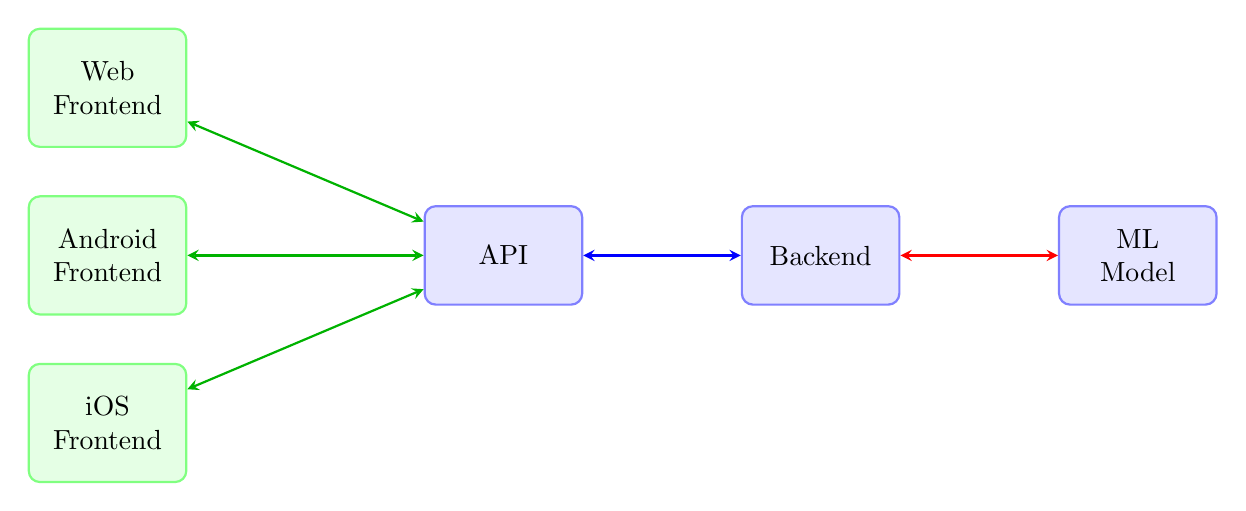
\begin{tikzpicture}[
    node distance=1.8cm,
    frontend/.style={rectangle, rounded corners, draw=green!50, fill=green!10, thick, minimum width=2cm, minimum height=1.5cm, align=center},
    backend/.style={rectangle, rounded corners, draw=blue!50, fill=blue!10, thick, minimum width=2cm, minimum height=1.25cm, align=center},
    arrow/.style={<->, >=stealth, thick}
]

% Frontends
\node[frontend] (web) {Web\\Frontend};
\node[frontend, below=0.6cm of web] (android) {Android\\Frontend};
\node[frontend, below=0.6cm of android] (ios) {iOS\\Frontend};

% API
\node[backend, right=3cm of android] (api) {API};

% Backend
\node[backend, right=2cm of api] (backend) {Backend};

% Model
\node[backend, right=2cm of backend] (model) {ML\\Model};

% Arrows
\draw[arrow, green!70!black] (web) -- (api);
\draw[arrow, green!70!black] (android) -- (api);
\draw[arrow, green!70!black] (ios) -- (api);
\draw[arrow, blue] (api) -- (backend);
\draw[arrow, red] (backend) -- (model);

\end{tikzpicture}
\end{center}

\textbf{Benefits:}
\begin{itemize}[leftmargin=*]
    \item One ML model
    \item One Backend
    \item One API
    \item Three separate Frontends
    \item All frontends use same recommender
    \item Consistent recommendations everywhere
\end{itemize}

\subsection{Industry Standard ML Architecture}

\begin{infobox}{Current Industry Practice}
\textbf{Standard ML Deployment Architecture:}

\vspace{0.5em}
When any company deploys an ML-based application:
\begin{enumerate}[leftmargin=*]
    \item Train ML/DL/Generative AI model
    \item Build Backend to interact with model
    \item Create API layer over Backend
    \item Develop platform-specific Frontends
    \item All Frontends consume same API
\end{enumerate}

\textbf{This is followed by:}
\begin{itemize}[leftmargin=*]
    \item Startups building AI products
    \item Large tech companies (Google, Microsoft)
    \item ML-focused companies (OpenAI, Anthropic)
    \item Any company deploying ML models
\end{itemize}
\end{infobox}

\subsection{Summary: APIs in ML Context}

\begin{infobox}{Key Takeaways}
\textbf{1. Similar Architecture:}
\begin{itemize}[leftmargin=*]
    \item ML APIs follow same pattern as Software APIs
    \item Only difference: Model instead of Database
    \item Same protocols (HTTP)
    \item Same data formats (JSON)
\end{itemize}

\textbf{2. Decoupling Benefits:}
\begin{itemize}[leftmargin=*]
    \item Model accessible to external applications
    \item Multiple platforms can use same model
    \item Easy integration and deployment
    \item Monetization opportunities
\end{itemize}

\textbf{3. Industry Standard:}
\begin{itemize}[leftmargin=*]
    \item Every ML product uses API architecture
    \item From ChatGPT to recommendation systems
    \item Essential for production deployment
    \item Critical skill for ML engineers
\end{itemize}
\end{infobox}

\newpage

% ========================
% SECTION 8: VIDEO SUMMARY
% ========================
\section{Summary and Next Steps}

\subsection{What We Learned Today}

\subsubsection{Main Topics Covered}

\hspace{1.5em}\textbf{1. What are APIs?}
\begin{itemize}[leftmargin=*]
    \item Mechanisms enabling software communication
    \item Act as connectors between applications
    \item Follow defined protocols and data formats
    \item Essential for modern application architecture
\end{itemize}

\textbf{2. Why APIs Exist?}
\begin{itemize}[leftmargin=*]
    \item Problem 1: External data access
    \begin{itemize}
        \item Monolithic apps couldn't share data
        \item APIs enable controlled external access
        \item Monetization opportunities
    \end{itemize}
    \item Problem 2: Multi-platform support
    \begin{itemize}
        \item Need for Web, Android, iOS apps
        \item Single Backend + API + Multiple Frontends
        \item Efficient architecture
    \end{itemize}
\end{itemize}

\textbf{3. APIs in Machine Learning}
\begin{itemize}[leftmargin=*]
    \item Same architecture principles apply
    \item Model replaces Database
    \item Backend interacts with Model
    \item API exposes prediction functionality
    \item Standard for ML deployment
\end{itemize}

\subsection{Key Concepts Recap}

\subsubsection{Monolithic vs API Architecture}

\begin{center}
\begin{tabular}{|p{0.45\textwidth}|p{0.45\textwidth}|}
\hline
\textbf{Monolithic} & \textbf{API-Based} \\
\hline
Everything in one application & Separate components \\
\hline
Tightly coupled & Loosely coupled \\
\hline
Cannot share externally & External access possible \\
\hline
Difficult to scale & Easy to scale \\
\hline
One platform only & Multi-platform support \\
\hline
Limited flexibility & Highly flexible \\
\hline
\end{tabular}
\end{center}

\subsubsection{API Communication}

\hspace{1.5em}\textbf{Protocol:} HTTP
\begin{itemize}[leftmargin=*]
    \item Standard Internet protocol
    \item Request-response model
    \item Used by all web-based APIs
\end{itemize}

\textbf{Data Format:} JSON
\begin{itemize}[leftmargin=*]
    \item Universal data format
    \item Language-independent
    \item Human-readable
    \item Machine-parseable
\end{itemize}

\subsection{Real-World Applications}

\begin{examplebox}{Use Cases Discussed}
\textbf{Software Domain:}
\begin{itemize}[leftmargin=*]
    \item IRCTC train information sharing
    \item Multi-platform applications (Web, Android, iOS)
    \item Third-party integrations
\end{itemize}

\textbf{ML Domain:}
\begin{itemize}[leftmargin=*]
    \item ChatGPT/GPT model access
    \item Recommender systems (Amazon)
    \item Chatbot improvements (Zomato)
    \item Review summarization (E-commerce)
    \item RAG systems (Document Q\&A)
\end{itemize}
\end{examplebox}

\end{document}